\documentclass[a4paper]{article}

%use the english line for english reports
%usepackage[english]{babel}
\usepackage[portuguese]{babel}
\usepackage[utf8]{inputenc}
\usepackage{indentfirst}
\usepackage{graphicx}
\usepackage{verbatim}
\usepackage{fancyhdr}
\usepackage{listings}
\usepackage{color}
\usepackage{hyperref}
\hypersetup{
    colorlinks=true,
    linkcolor=blue,
    filecolor=magenta,      
    urlcolor=cyan,
}

\definecolor{dkgreen}{rgb}{0,0.6,0}
\definecolor{gray}{rgb}{0.5,0.5,0.5}
\definecolor{mauve}{rgb}{0.58,0,0.82}

\lstset{frame=tb,
  language=Prolog,
  aboveskip=3mm,
  belowskip=3mm,
  showstringspaces=false,
  columns=flexible,
  basicstyle={\small\ttfamily},
  numbers=none,
  numberstyle=\tiny\color{gray},
  keywordstyle=\color{blue},
  commentstyle=\color{dkgreen},
  stringstyle=\color{mauve},
  breaklines=true,
  breakatwhitespace=true,
  tabsize=3
  }

\begin{document}


\setlength{\textwidth}{16cm}
\setlength{\textheight}{22cm}

\title{\Huge\textbf{FABRIK}\linebreak\linebreak\linebreak
\Large\textbf{Manual do Utilizador}\linebreak\linebreak
\linebreak\linebreak

\includegraphics[scale=0.1]{images/feup-logo.png}\linebreak\linebreak
\linebreak\linebreak
\Large{Mestrado Integrado em Engenharia Informática e Computação} \linebreak\linebreak
\Large{Laboratório de Aplicações com Interface Gráfica}\linebreak
}

\author{\textbf{Turma 1, Grupo 7}\\
\linebreak\\
André Cruz - 201503776 \\
Edgar Carneiro - 201503748 \\
\linebreak\linebreak \\
 \\ Faculdade de Engenharia da Universidade do Porto \\ Rua Roberto Frias, s\/n, 4200-465 Porto, Portugal \linebreak\linebreak\linebreak
\linebreak\linebreak\vspace{1cm}}

\maketitle
\thispagestyle{empty}

%************************************************************************************************
%************************************************************************************************

\newpage


\tableofcontents

%************************************************************************************************
%************************************************************************************************

%*************************************************************************************************
%************************************************************************************************

\newpage

%%%%%%%%%%%%%%%%%%%%%%%%%%
\section{\textit{Set-Up}}

Para correr o cliente (interface gráfica) basta correr o script ‘start\_client.sh’:
\begin{itemize}
\item \verb|sh start_client.sh|
\end{itemize}

No caso de não ser possível correr shell scripts terá de correr o comando ‘python -m http.server 8080’ manualmente.
\\
\\
Para correr o servidor de prolog terá de correr o script ‘start\_server.sh’:
\begin{itemize}
\item \verb|sh start_server.sh|
\end{itemize}

No caso de não ser possível correr shell scripts terá de abrir o Sicstus, consultar o ficheiro de Prolog server.pl - consult(‘server.pl’). - e de seguida correr o predicado server.

Após ter iniciado o servidor http e o servidor de prolog, basta navegar até à página ‘localhost:8080/client’ para correr o jogo.


\newpage

%%%%%%%%%%%%%%%%%%%%%%%%%%
\section{O Jogo \textit{Fabrik}}

\subsection{História}
O jogo - \textit{Fabrik} - foi recentemente desenvolvido por Dieter Stein, em agosto de 2017, como parte de um estudo para o desenvolvimento de um novo jogo, Urbino.

\subsection{Material}
\begin{itemize}
	\item Tabuleiro quadrangular
	\item Quantidade suficiente de peças pretas e brancas
	\item Duas peças vermelhas chamadas trabalhadores
\end{itemize}

\begin{figure}[h!]
\begin{center}
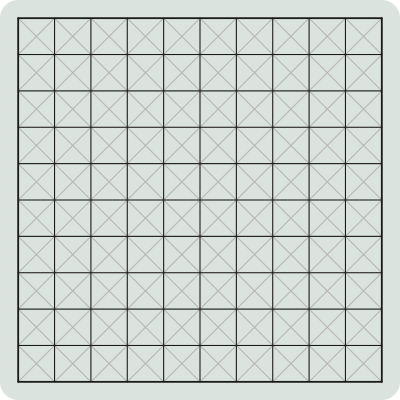
\includegraphics[height=3cm,width=3cm]{images/fabrik_empty_board.png}
\caption{Tabuleiro vazio de 11 x 11 espaços}
\end{center}
\end{figure}

\subsection{Regras}
A implementação deste jogo foi baseada no manual de regras oficiais, disponível em \href{https://spielstein.com/games/fabrik}{https://spielstein.com/games/fabrik}.

As pretas (jogador que joga com peças de cor preta) começam por colocar um dos trabalhadores num espaço à sua escolha. De seguida, as brancas (jogador que joga com peças de cor branca) colocam o outro trabalhador num espaço livre. De seguida, as pretas decidem quem começa por jogar.

O jogo procede por turnos, sendo que em cada turno um jogador pode, se assim optar, mover um dos trabalhadores para um espaço vazio. De seguida, o jogador deve jogar colocar uma das suas peças num ponto de interseção entre as “linhas de visão dos dois trabalhadores”. As linhas de visão dos trabalhadores são as linhas na diagonal, horizontal e vertical sobre as quais os trabalhadores se encontram posicionados.

\begin{figure}[h!]
\begin{center}
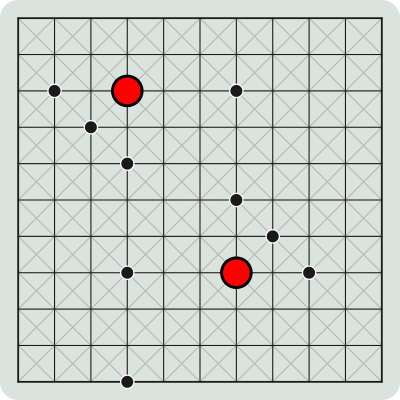
\includegraphics[height=3cm,width=3cm]{images/fabrik_intersection.png}
\caption{Pontos de interseção entre os dois trabalhadores}
\end{center}
\end{figure}

No caso especial em que os dois trabalhadores se encontram sobre uma mesma linha ortogonal ou diagonal, apenas os espaços entre eles são considerados pontos de interseção (se estiverem vazios), ao invés da totalidade dessa linha.

Ganha o jogo o jogador que consiga criar uma linha de pelo menos 5 pedras da sua cor, ortogonal ou diagonalmente. Um jogador ganha também o jogo se o seu adversário não conseguir posicionar nenhum dos trabalhadores de forma a poder colocar uma pedra sua no tabuleiro.

\begin{figure}[h!]
\begin{center}
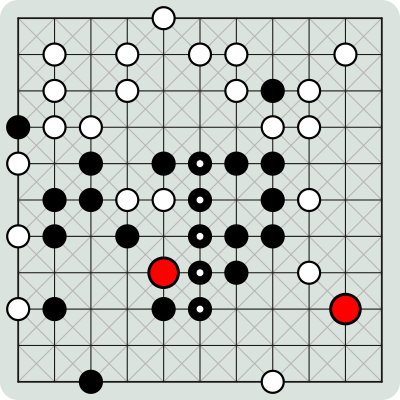
\includegraphics[height=3cm,width=3cm]{images/fabrik_full_board.png}
\caption{Final de uma partida de Fabrik, com vitórias das pretas}
\end{center}
\end{figure}

\newpage

%%%%%%%%%%%%%%%%%%%%%%%%%%
\section{Instruções de Uso}

Como podemos ver pela figura 4 (disponível na última página), foram implementadas todas as funcionalidades requeridas no enunciado do trabalho. É possível fazer a mudança entre as diferentes cenas carregadas através de diferentes XML’s, sendo para tal apenas necessário mudar qual a cena a ser displayed usando a dropdown box presente no início da interface.

Foram implementados também três diferentes modos de jogo: humano contra humano, humano contra computador e computador contra computador. Foram também implementadas duas dificuldades para os jogos de computador: dificuldade Dummy, caracterizada por jogadas aleatórias por parte do computador, e dificuldade Smart em que o computador, usando um algoritmo ganancioso por nós concebido, avalia todos os tabuleiros possíveis e escolhe o por ele considerado melhor.  Assim, é possível, no modo Singleplayer jogar contra um computador Smart ou Dummy. No modo computador contra computador, é possível escolher um jogo de entre as 4 combinações possíveis: Smart x Smart, Smart x Dummy, Dummy x Smart e Dummy x Dummy.

Em relação ao grupo ‘Opções’ da interface, este permite ao utilizador interagir com o jogo, permitindo-lhe realizar as seguintes funcionalidades: anular a última jogada feita, sendo que se depois voltar a carregar anula a jogada anterior a essa e assim consequentemente; ver o filme de jogo, que repete em modo animação todas as jogada realizadas desde o início do jogo, sendo que esta funcionalidade pode ser ativada a qualquer momento; terminar com o jogo, terminando assim o jogo empatado, e, finalmente, escolher qual a cor do shader aplicado aos trabalhadores quando estes são clicados. Qualquer uma destas funcionalidades pode ser aplicada em qualquer modo, continuando o programa a fluir naturalmente.

Em relação ao grupo ‘Câmara’ da interface, este permite ao utilizador variar o seu ponto de vista. É permitido fazer zoom in  ou zoom out da cena e é permitido, rodar a câmara entre 4 posições definidas. Fazer zoom out permite também ao utilizador ter uma melhor perceção da cena que o rodeia. De destacar que a transição entre posições é sempre feita com recurso a animações visualmente agradáveis e naturais.

Por fim, o grupo das ‘luzes’ permite ao utilizador activar quais as luzes que quer que estejam ativas. Naturalmente, que este grupo conforma a cena a ser displayed no momento.

Em relação, à cena, para movimentação de peças, no início do jogo, na fase de escolha da posição inicial dos trabalhadores, apenas é necessário carregar nas célula destino. Passa a fase inicial, para movimentação de um trabalhador, carrega-se neste e de seguida numa célula do tabuleiro livre. Para a posição de peças, não estando um trabalhador selecionado, carregando numa célula válida, uma peça mover-se-à, segunda uma animação, para essa posição. Naturalmente, foram implementados para lidar com seleção de peças inválidas.
Adicionalmente, existe uma peça animada que se mexe no tabuleiro, por uma das bordas, que tem como fim indicar de quem é o turno de jogo: se do lado das pretas, é das pretas, se do lado das brancas, é das brancas.

Por fim, para controlo do tempo de jogo, é utilizado um placar, que indica qual a pontuação de cada jogador e qual o tempo restante em cada turno. Se o temporizador começar a 0:00, não existe tempo limite para cada jogo. Para alterar esse valor, o utilizador deve clicar ou no número das dezenas dos segundos ou no número dos minutos, incrementando assim o relógio em 10s ou 1min, respetivamente. Caso um jogador não faça a sua jogada a tempo, perde. Os restantes números do placar, de cada lado do temporizador, indicando a pontuação de cada um dos jogadores.

\begin{figure}[p]
\begin{center}
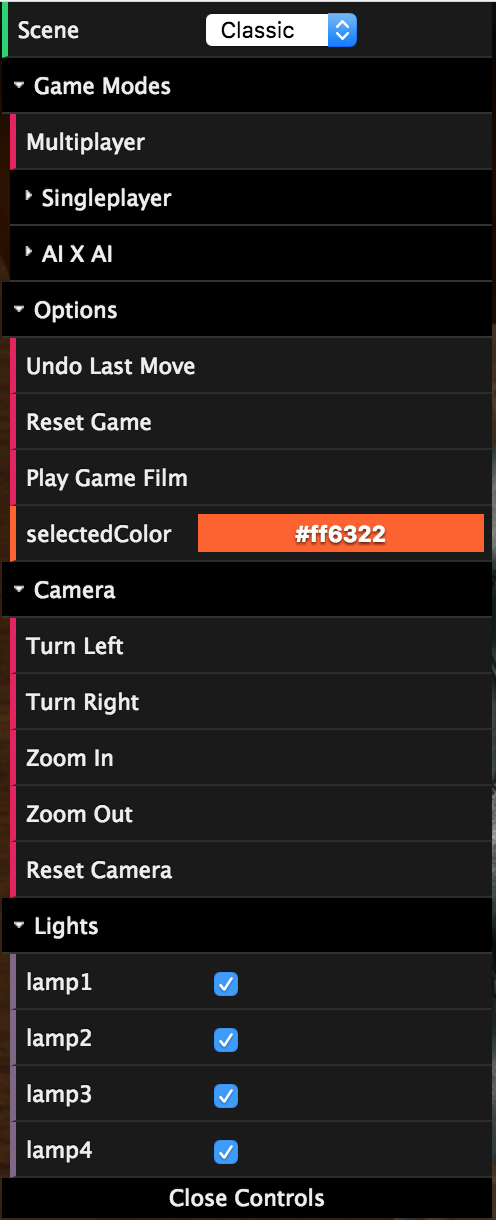
\includegraphics[scale=0.5]{images/interface.png}
\caption{Interface do Jogo}
\end{center}
\end{figure}

\begin{figure}[p]
\begin{center}
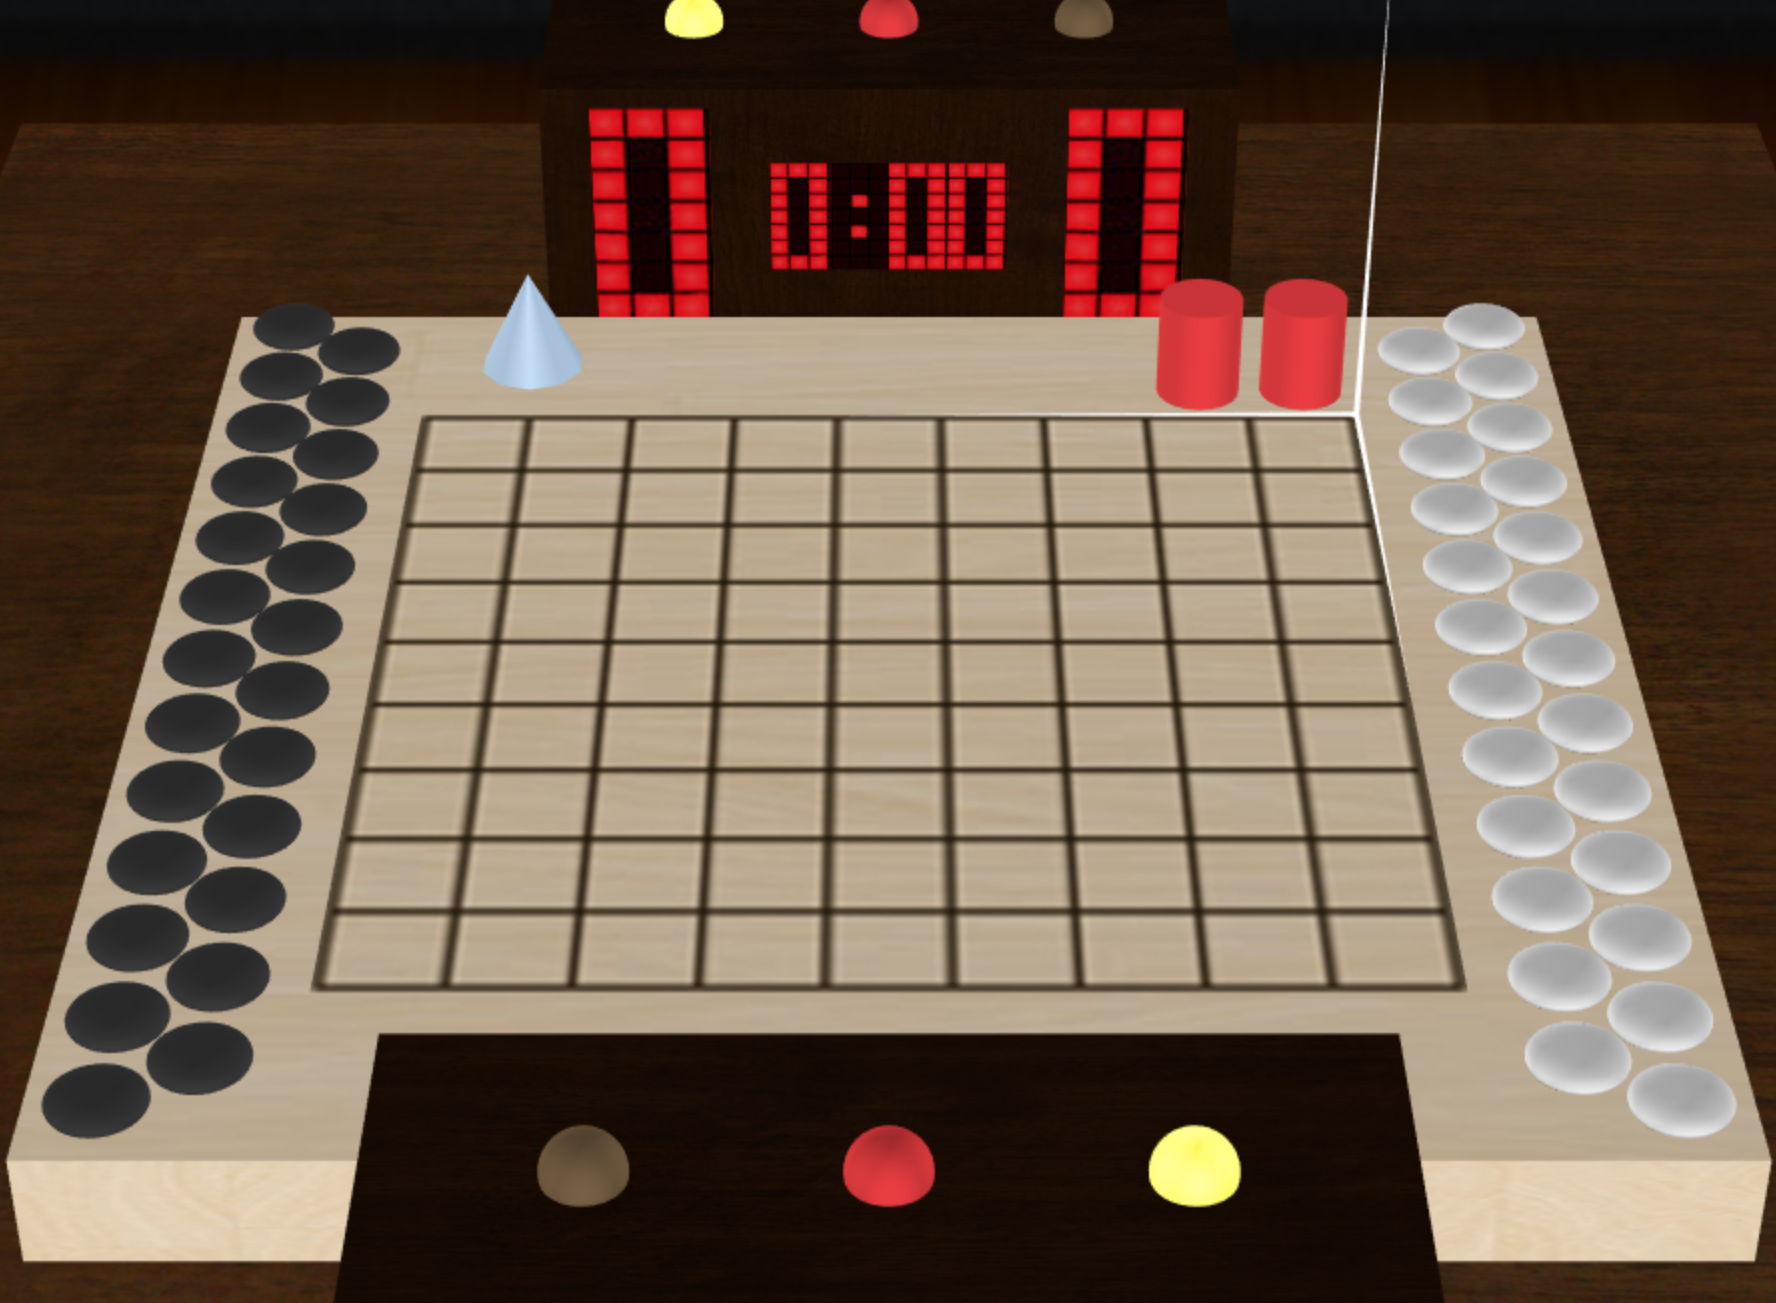
\includegraphics[scale=0.4]{images/screenshot.png}
\caption{Visualização geral do jogo.}
\end{center}
\end{figure}

\newpage

\end{document}
